\documentclass{beamer}

\usepackage[english]{babel}
\usepackage[utf8x]{inputenc}
\usepackage[T1]{fontenc}
\usepackage{lmodern}
\usepackage{hus-beamer} 
%------ tikZ ------%
\usepackage{tikz}
\usetikzlibrary{positioning, arrows}
\usetikzlibrary{backgrounds}

\mode<presentation>{
	\usefonttheme{professionalfonts} % normal font for math formulas
	% insert section page with title only
	% before each section
	\AtBeginSection[]{
	\begin{frame}%[noframenumbering] % remove this if you do not want to number section page
	\vfill
	\centering
	\begin{beamercolorbox}[sep=8pt,center,shadow=true,rounded=true]{title}
	\usebeamerfont{title}\insertsectionhead\par%
	\end{beamercolorbox}
	\vfill
	\end{frame}
}
}

%------------------%
\usepackage{ifthen}
\begin{document}
\title{Convolution Neural Networks}
\subtitle{Week 3}
\author{COMP6252 (Deep Learning Technologies)}
\institute[ECS, University of Southampton]{ECS, University of Southampton} \date{28 April 2022}

\begin{frame}[plain,noframenumbering]
    \placelogofalse % No logo at the title page
    \titlepage
\end{frame}
    
\placelogotrue
\begin{frame}
    \frametitle{Introduction}
    \begin{itemize}
    \item A convolution network usually has at least one convolution layer
    \item A convolution operation (slightly different from the usual definitio) is done by multiplying weights element-wise with a portion of the input
    \item The same operation with the same weights is repeated over all the input
    \item The set of weights are usually referred to as the \textbf{kernel}
    \item The result of the convolution is referred to as the \textbf{feature map} or \textbf{activation map}
    \end{itemize}
  \end{frame}
\begin{frame}
    \frametitle{Convolution operation on an input image with 3 channels (RGB)}
    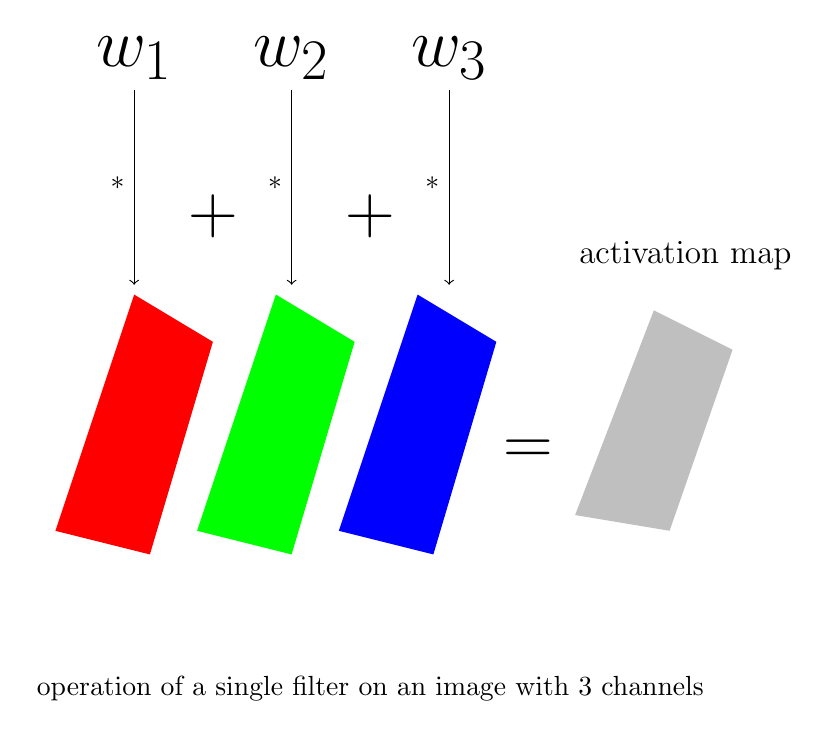
\begin{tikzpicture}
        \node (w1) at (1,6) {\Huge $w_1$};
        \node (w2) at (3,6) {\Huge $w_2$};
        \node (w3) at (5,6) {\Huge $w_3$};
        \node (anc1) at (1,3) {};
        \node (anc2) at (3,3) {};
        \node (anc3) at (5,3) {};
        \node (add1) at (2,4) {\Huge +};
        \node (add2) at (4,4) {\Huge +};
    
        \path[->] (w1) edge node[left]{*} (anc1);
        \path[->] (w2) edge node[left]{*} (anc2);
        \path[->] (w3) edge node[left]{*} (anc3);
    
        \coordinate (a) at (0,0);
         \coordinate (b) at (1,3);
         \coordinate (c) at (2,2.4);
         \coordinate (d) at (1.2,-0.3);
        \filldraw[draw=none,fill=red] (a) -- (b) -- (c) -- (d) -- (a);
    
    
        \coordinate (a1) at (1.8,0);
        \coordinate (b1) at (2.8,3);
        \coordinate (c1) at (3.8,2.4);
        \coordinate (d1) at (3,-0.3);
       \filldraw[draw=none,fill=green] (a1) -- (b1) -- (c1) -- (d1) -- (a1);
        %\filldraw[fill=red] (a) circle (2);
    
        \coordinate (a2) at (3.6,0);
        \coordinate (b2) at (4.6,3);
        \coordinate (c2) at (5.6,2.4);
        \coordinate (d2) at (4.8,-0.3);
       \filldraw[draw=none,fill=blue] (a2) -- (b2) -- (c2) -- (d2) -- (a2);
        %\filldraw[fill=red] (a) circle (2);
    
    \node (eq) at (6,1) {\Huge =};
        \coordinate (a3) at (6.6,0.2);
        \coordinate (b3) at (7.6,2.8);
        \coordinate (c3) at (8.6,2.3);
        \coordinate (d3) at (7.8,0);
       \filldraw[draw=none,fill=lightgray] (a3) -- (b3) -- (c3) -- (d3) -- (a3);
       \node (label) at (4,-2) {operation of a single filter on an image with 3 channels};
       \node (amap) at (8,3.5) {\large activation map};
    \end{tikzpicture}
    

\end{frame}
\begin{frame}[c]
\frametitle{Conv operation on one channel}
\begin{center}
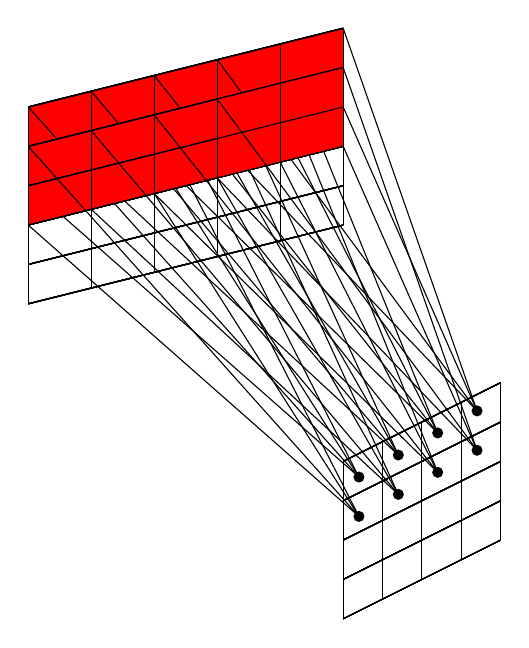
\begin{tikzpicture}
\pgfmathtruncatemacro\N{10}
\foreach \j in {1,...,8}{
    \onslide<\j>{
        \pgfmathsetmacro{\dx}{
            \j<5 ? (0.8*(\j-1)): (0.8*(\j-5))
            }
        \pgfmathsetmacro{\dy}{
            \j<5 ? (0.2*(\j-1)): (0.2*(\j-5)-0.5)
            }
        \pgfmathsetmacro{\tmp}{
            \j<5 ? (8) : (9)
        }
        %\begin{scope}[on background layer]
            \coordinate (a) at (0+\dx,3+\dy);
            \coordinate (d) at (0+\dx ,2+ \dy);
            \coordinate (b) at (1.6+\dx ,3.4+\dy);
            \coordinate (c) at (1.6+\dx,2.4+ \dy);
            \filldraw[fill=red,draw=none] (a) -- (b) -- (c) -- (d) --(a);
        %\end{scope}
        %\node[rectangle,draw] (r) at (\j,\j) {};

          \foreach \k in {1,...,6}
          {
          \pgfmathsetmacro{\idx}{0.2*(\k-1)}
          \pgfmathsetmacro{\sep}{0.8*(\k-1)}


          %horizontal lines
          \path[draw] (0,0.5*\k) -- (4,0.5*\k+1);
          %vertical lines
          \path[draw] (\sep,3+\idx) -- (\sep,0.5+\idx);

          }
          \foreach \k in {1,...,5}
          {
          \pgfmathsetmacro{\idx}{0.25*(\k-1)}
          \pgfmathsetmacro{\sep}{0.5*(\k-1)}


          %horizontal lines
          \path[draw] (4,0.5*\k-4) -- (6,0.5*\k+1-4);
          %vertical lines
          \path[draw] (4+\sep,-1.5+\idx) -- (4+\sep,-3.5+\idx);

          }
          \pgfmathsetmacro{\ccx}{
            \j<5 ? (4.2+0.5*(\j-1)): (4.2+0.5*(\j-5))
            }
            \pgfmathsetmacro{\ccy}{
                \j<5 ? (-1.7+0.28*(\j-1)): (-2.2+0.28*(\j-5))
                }
          \fill (\ccx,\ccy) circle (2pt);
          \path[draw] (a) -- (\ccx,\ccy);
          \path[draw] (b) -- (\ccx,\ccy);
          \path[draw] (c) -- (\ccx,\ccy);
          \path[draw] (d) -- (\ccx,\ccy);
    }
}

\end{tikzpicture}
\end{center}

\end{frame}


%% bottom part
\begin{frame}[c]
    \frametitle{Conv operation on one channel}
    \begin{center}
    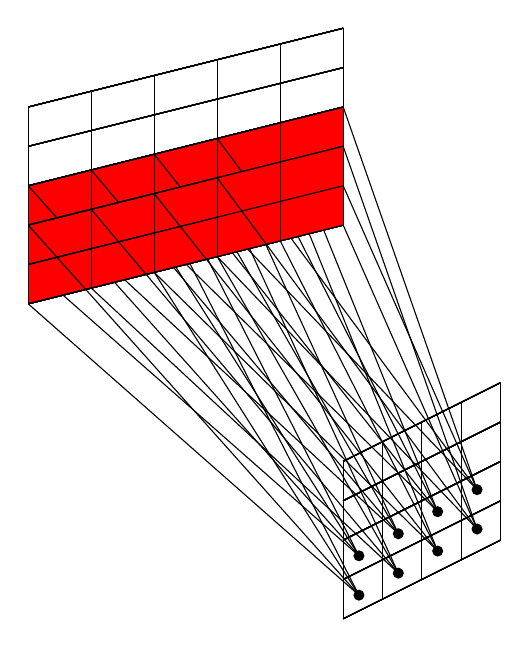
\begin{tikzpicture}
    \pgfmathtruncatemacro\N{10}
    \foreach \j in {1,...,8}{
        \onslide<\j>{
            \pgfmathsetmacro{\dx}{
                \j<5 ? (0.8*(\j-1)): (0.8*(\j-5))
                }
            \pgfmathsetmacro{\dy}{
                \j<5 ? (0.2*(\j-1)): (0.2*(\j-5)-0.5)
                }
            \pgfmathsetmacro{\tmp}{
                \j<5 ? (8) : (9)
            }
                \coordinate (a) at (0+\dx,2+\dy);
                \coordinate (d) at (0+\dx ,1+ \dy);
                \coordinate (b) at (1.6+\dx ,2.4+\dy);
                \coordinate (c) at (1.6+\dx,1.4+ \dy);
                \filldraw[fill=red,draw=none] (a) -- (b) -- (c) -- (d) --(a);
          
              \foreach \k in {1,...,6}
              {
              \pgfmathsetmacro{\idx}{0.2*(\k-1)}
              \pgfmathsetmacro{\sep}{0.8*(\k-1)}
    
    
              %horizontal lines
              \path[draw] (0,0.5*\k) -- (4,0.5*\k+1);
              %vertical lines
              \path[draw] (\sep,3+\idx) -- (\sep,0.5+\idx);
    
              }
              \foreach \k in {1,...,5}
              {
              \pgfmathsetmacro{\idx}{0.25*(\k-1)}
              \pgfmathsetmacro{\sep}{0.5*(\k-1)}
    
    
              %horizontal lines
              \path[draw] (4,0.5*\k-4) -- (6,0.5*\k+1-4);
              %vertical lines
              \path[draw] (4+\sep,-1.5+\idx) -- (4+\sep,-3.5+\idx);
    
              }
              \pgfmathsetmacro{\ccx}{
                \j<5 ? (4.2+0.5*(\j-1)): (4.2+0.5*(\j-5))
                }
                \pgfmathsetmacro{\ccy}{
                    \j<5 ? (-2.7+0.28*(\j-1)): (-3.2+0.28*(\j-5))
                    }
              \fill (\ccx,\ccy) circle (2pt);
              \path[draw] (a) -- (\ccx,\ccy);
              \path[draw] (b) -- (\ccx,\ccy);
              \path[draw] (c) -- (\ccx,\ccy);
              \path[draw] (d) -- (\ccx,\ccy);
        }
    }
    
    \end{tikzpicture}
    \end{center}
    
    \end{frame}
    

    \begin{frame}
        \frametitle{Example: Conv. operation on one channel}
      \vspace{-1cm}
      
      
          \begin{tabular}[h]{|c|c|c|c|}
            \multicolumn{4}{c}{Input}\\
            \hline
             {\only<1>{\color{red}} 1}& {\only<1-2>{\color{red}} 2} &  {\only<2-3>{\color{red}} 4}&  {\only<3>{\color{red}} 3}\\
            \hline
               {\only<1,4>{\color{red}} 5}&{\only<1-2,4-5>{\color{red}} 6}& {\only<2-3,5-6>{\color{red}} 8}&{\only<3,6>{\color{red}} 7}\\
           \hline
               {\only<4,7>{\color{red}} 9}&{\only<4-5,7-8>{\color{red}} 10}  &{\only<5-6,8-9>{\color{red}} 12}&{\only<6,9>{\color{red}} 11}\\
           \hline
              {\only<7>{\color{red}} 13}&{\only<7-8>{\color{red}} 14} &{\only<8-9>{\color{red}} 16} &{\only<9>{\color{red}} 2}\\
           \hline
          \end{tabular}
      \hspace{0.5cm}$\odot$\hspace{0.5cm}
          \begin{tabular}[h]{|c|c|}
            \multicolumn{2}{c}{Kernel}\\
            \hline
             1 &-2 \\
            \hline
             -3 & 4\\
             \hline
          \end{tabular}
      
      
      \vspace{1cm}
      \hspace{4.5cm}
      =
      %\onslide<2>{
      \begin{tabular}[h]{|c|c|c|}
        \hline
         \only<1-> 6& \only<2-> 8 &\only<3-> {2}\\
        \hline
        \only<4-> 6  &\only<5-> 8 &\only<6->2\\
        \hline
        \only<7-> 6 &\only<8-> 8 &\only<9-> {-50}\\
        \hline
      \end{tabular}
      \tikz{
        \node[overlay] at (-1,1.2) {activation map};

      }
      
      \end{frame}

   \begin{frame}
    \frametitle{Add stride 2 example here}
   
    
   
   \end{frame}   
\begin{frame}
    \frametitle{Stride and receptive field}
\begin{itemize}
    \item In the previous example we used a \textbf{stride} equal to 1
    \item The kernel \textbf{receptive field} was equal to 2x2
    \item The size of the output (activation map) was 3x3
    \item Are those numbers the same in all applications? No
\end{itemize}
    

\end{frame}  
\begin{frame}
    \frametitle{Stride and receptive field}
\begin{itemize}
    \item In general one can use a stride of any size $S$. Stride of size 1 is the most common.
    \item Let $F\times F$ be the kernel \textbf{receptive field} 
    \item Let $H_i\times W_i\times C_i$ be the size of the input
    \item The size of the resulting activation map is $H_o\times W_o$ where 
    \begin{align*}
        H_o&=\left\lfloor\frac{H_i-F}{S}\right\rfloor+1\\
        W_o&=\left\lfloor\frac{W_i-F}{S}\right\rfloor+1
    \end{align*}
\end{itemize}
\end{frame}  
\begin{frame}
    \frametitle{Example}
    \begin{itemize}
        \item Consider an input image of size (3,28,28)
        \item We are using the PyTorch convention with the channel dimension first.
        \item What would be the size of the activation map if a kernel of size 3x3 and stride 2 were used?

        \item Height and width are the same and equal to $\left\lfloor\frac{28-3}{2}\right\rfloor+1=13$
        \item So the activation map has size 13x13
        \item Note that the output of \textbf{one} kernel is a 2-d object: the activation map.
        \item The number of output channels is determined by the \textbf{number} of kernels
    \end{itemize}
\end{frame}
\begin{frame}
    \frametitle{Parameters}
    \begin{itemize}
        \item Consider an image of size (3,28,28) used as input to 32 filters of size 3x3
        \item Since the input has 3 channels each filter has 3x3x3+1(bias)=28 Parameters
        \item With a stride of 1 the output has size (32,26,26), i.e., the layer has 32x26x26=21632 nodes
        \item Total number of parameters=32x28=896
        \item Contrast the above with a feedforward with the first layer having 32x26x26=21632 nodes
        \item It would have (3x28x28)*21632=50878464 parameters !(without bias)
    \end{itemize}
    

\end{frame}
\begin{frame}
    \frametitle{Padding}
    \begin{itemize}
        \item We saw previously that convolution reduces the size of the input
        \item When multiple layers are used the size is reduced at each layer
        \item Sometimes we don't want the size to change
        \item more importantly the "edges" of the input do not contribute as much as the "middle"
        \item One solution is to pad the input with zeros.
    \end{itemize}
\end{frame}

\begin{frame}
    \frametitle{Zero padding}
\begin{columns}
\begin{column}{0.5\textwidth}
    \begin{tabular}[h]{|c|c|c|}
        \multicolumn{3}{c}{Input}\\
        \hline
         1& 2 &1 \\
         \hline
         4 & 2 & 3 \\
         \hline
         2 & 1 & 1\\
        \hline
    \end{tabular}

    
\end{column}
\begin{column}{0.5\textwidth}
    \begin{tabular}[h]{|c|c|c|c|c|}
        \multicolumn{5}{c}{0 padded}\\
        \hline
        {\color{red}0} & {\color{red}0} & {\color{red}0} & {\color{red}0} &{\color{red}0}\\
        \hline
        {\color{red}0} & 1& 2 &1 & {\color{red}0}\\
         \hline
         {\color{red}0}&  4 & 2 & 3 & {\color{red}0} \\
         \hline
         {\color{red}0}& 2 & 1 & 1 & {\color{red}0}\\
        \hline
        {\color{red}0} & {\color{red}0} & {\color{red}0} & {\color{red}0} & {\color{red}0}\\
        \hline
    \end{tabular}
\end{column}

\end{columns}
    \begin{itemize}
        \item The output size in the presence of padding
   
    \begin{align*}
        H_o&=\left\lfloor\frac{H_i+2P-F}{S}\right\rfloor+1\\
        W_o&=\left\lfloor\frac{W_i+2P-F}{S}\right\rfloor+1
    \end{align*}
    \item  Same formula as before if we consider the \textbf{effective} height =$H_i+2P$ and width=$W_i+2P$ 
\end{itemize}
\end{frame}

\begin{frame}
    \frametitle{Convolution operation mathematically}
\begin{itemize}
    \item Let $f,i,j$ be the filter index,output height index, and output width respectively
    \item For a stride of 1 (most common), and bias per filter $b_f$
    \item The convolution operation is defined as
    
\begin{align*}
O_{f,i,j}=b_f+\sum_c\sum_{m,n}X_{c,i+m,j+n}*K_{f,c,m,n}
\end{align*}
\item If one includes the sample index $s$, needed in the case of batches
\begin{align*}
    O_{s,f,i,j}=b_f+\sum_c\sum_{m,n}X_{s,c,i+m,j+n}*K_{f,c,m,n}
    \end{align*}
\end{itemize}

\end{frame}
\begin{frame}
    \frametitle{Pooling}

    \begin{itemize}
        \item Typically, convolutional networks performs three steps 
        \begin{enumerate}
            \item Convolution operation
            \item followed by a Non-linear activation such as ReLU 
            \item followed by \textbf{pooling}
        \end{enumerate}
\item Pooling computes a summary statistics for a small area of the result
\item Taking the max value is the most common pooling operation.
    \end{itemize}

\end{frame}
\begin{frame}[c]
    \frametitle{Pooling size 2x2, stride=2}
    \begin{center}
    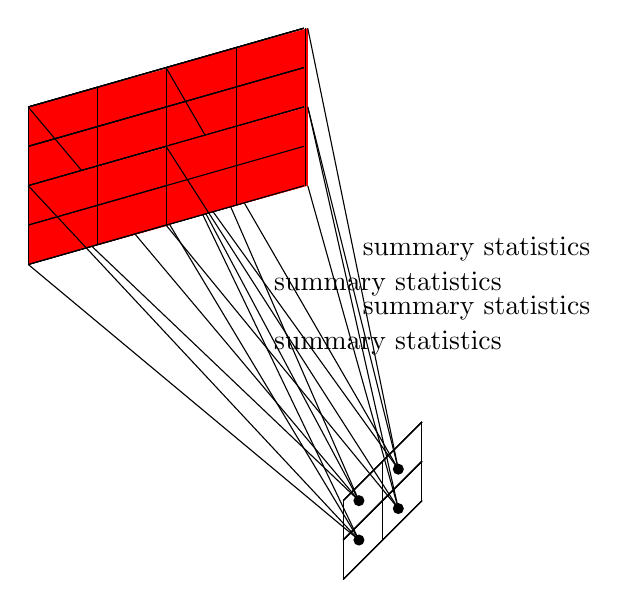
\begin{tikzpicture}
    \pgfmathtruncatemacro\N{10}
    \foreach \j in {1,...,4}{
        \onslide<\j>{
            \pgfmathsetmacro{\dx}{
                \j<3 ? (1.75*(\j-1)): (1.75*(\j-3))
                }
            \pgfmathsetmacro{\dy}{
                \j<3 ? (0.5*(\j-1)): (0.5*(\j-3)-1.)
                }
            \pgfmathsetmacro{\tmp}{
                \j<5 ? (8) : (9)
            }
                \coordinate (a) at (0+\dx,2.5+\dy);
                \coordinate (d) at (0+\dx ,1.5+ \dy);
                \coordinate (b) at (1.8+\dx ,3+\dy);
                \coordinate (c) at (1.8+\dx,2+ \dy);
                \filldraw[fill=red,draw=none] (a) -- (b) -- (c) -- (d) --(a);
          
              \foreach \k in {1,...,5}
              {
              \pgfmathsetmacro{\idx}{0.25*(\k-1)}
              \pgfmathsetmacro{\sep}{0.88*(\k-1)}
    
    
              %horizontal lines
              \path[draw] (0,0.5*\k) -- (3.5,0.5*\k+1);
              %vertical lines
              \path[draw] (\sep,2.5+\idx) -- (\sep,0.5+\idx);
    
              }
              \foreach \k in {1,...,3}
              {
              \pgfmathsetmacro{\idx}{0.5*(\k-1)}
              \pgfmathsetmacro{\sep}{0.5*(\k-1)}
    
    
              %horizontal lines
              \path[draw] (4,0.5*\k-4) -- (5,0.5*\k+1-4);
              %vertical lines
              \path[draw] (4+\sep,-2.5+\idx) -- (4+\sep,-3.5+\idx);
    
              }
              \pgfmathsetmacro{\ccx}{
                \j<3 ? (4.2+0.5*(\j-1)): (4.2+0.5*(\j-3))
                }
                \pgfmathsetmacro{\ccy}{
                    \j<3 ? (-2.5+0.4*(\j-1)): (-3.+0.4*(\j-3))
                    }
              \fill (\ccx,\ccy) circle (2pt);
              \path[draw] (a) edge (\ccx,\ccy) ;
              \path[draw] (b) edge [right] node {summary statistics} (\ccx,\ccy);
              \path[draw] (c) edge (\ccx,\ccy);
              \path[draw] (d) -- (\ccx,\ccy);
        }
    }
    
    \end{tikzpicture}
    \end{center}
    
\end{frame}

\begin{frame}
    \frametitle{Max pooling}

    \begin{tabular}[h]{|c|c|c|c|}
        \multicolumn{4}{c}{Input}\\
        \hline
         {\only<1>{\color{red}} 1}& {\only<1>{\color{red}} 2} &  {\only<2>{\color{red}} 4}&  {\only<2>{\color{red}} 3}\\
        \hline
           {\only<1>{\color{red}} 5}&{\only<1>{\color{red}} 6}& {\only<2>{\color{red}} 8}&{\only<2>{\color{red}} 7}\\
       \hline
           {\only<3>{\color{red}} 9}&{\only<3>{\color{red}} 10}  &{\only<4>{\color{red}} 12}&{\only<4>{\color{red}} 11}\\
       \hline
          {\only<3>{\color{red}} 13}&{\only<3>{\color{red}} 14} &{\only<4>{\color{red}} 16} &{\only<4>{\color{red}} 2}\\
       \hline
      \end{tabular}
   \hspace{0.5cm}Max Pool=\hspace{0.5cm}

  
  \vspace{-2cm}
  \hspace{7cm}
  %\onslide<2>{
  \begin{tabular}[h]{|c|c|}
    \hline
     \only<1-> {6} & \only<2-> {8} \\
    \hline
    \only<3-> {14} &\only<4-> {16}\\
    \hline
  \end{tabular}
  \tikz{
    \node[overlay] at (-1,1.2) {Result};

  }
  

\end{frame}
\end{document}